\section{Auswertung}
\label{sec:Auswertung}
Mit der Wheatoneschen Brückenschaltung sollten zwei Unbekannte Widerstände ermittelt werden.
\begin{table}
  \centering
  \caption{Messdaten der Widerstände $R_2$, $R_3$ und $R_4$, für $R_\text{x}$= Wert 10 und $R_\text{x}$= Wert 11.}
  \label{tab:widerstand}
  \sisetup{table-format=4}
  \begin{tabular}{c S S[table-format=3.1] S[table-format=3.1] S S S}
    \toprule
    &\multicolumn{3}{c}{{Wert 10}} & \multicolumn{3}{c}{{Wert 11}} \\
    \cmidrule(lr){2-4}\cmidrule(lr){5-7}
    {\,} & {$R_2 \mathbin{/} \si{\ohm}$} & {$R_3 \mathbin{/} \si{\ohm}$} & {$R_4 \mathbin{/} \si{\ohm}$} &{$R_2 \mathbin{/} \si{\ohm}$} 
    & {$R_3 \mathbin{/} \si{\ohm}$} & {$R_4 \mathbin{/} \si{\ohm}$}\\
    \midrule
   Messung 1 &332 & 420 & 580 & 332 &597 & 403\\
   Messung 2 & 664 & 264 & 736 &664 & 424 & 576\\
   Messung 3 &1000 & 193.5 & 806.5 &1000 & 330 & 670\\
    \bottomrule
  \end{tabular}
\end{table}
Mit den Messwerten aus \ref{tab:widerstand}, lässt sich mit Hilfe der Formel II der Widerstand $R_\text{x}$ berechnen.
Als Ergebniss erhält man für den Wert 10:
  \begin{align*}
  R_\text{x}&=240.41 & R_\text{x}&=240.41 \\
  R_\text{x}&=238.17 & R_\text{x}&=238.17 \\
  R_\text{x}&=239.93 & R_\text{x}&=239.93
\end{align*}
\begin{figure}
  \centering
  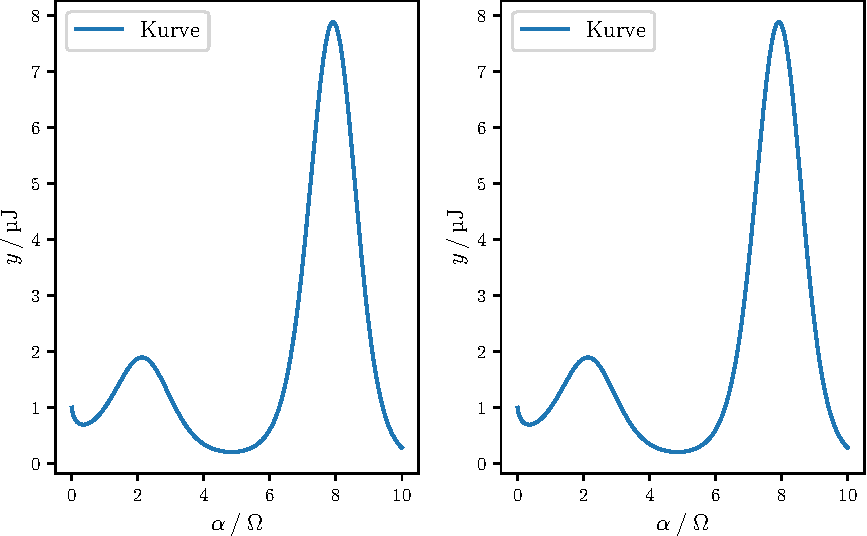
\includegraphics{plot.pdf}
  \caption{Plot.}
  \label{fig:plot}
\end{figure}


Siehe \autoref{fig:plot}!
